\section{A Semiotic Approach of Agents and Communication}

\subsection{An Overview of Feature Terms}\label{sec:FT}

Our protocol of argumentation is based on the capacity of agents to associate a semiotic elements from any type with a given set of examples -- the adjunct set. While this capacity can be granted by various approaches in machine learning -- as long as they can be interpreted as generalizing over and classifying examples, we will mostly focus on the use of feature terms to associate the semiotic elements with their adjunct sets.

Feature terms, also called feature structures or $\psi$-terms, are a generalization of first-order terms that have been introduced in theoretical computer science in order to formalize object-oriented capabilities of declarative languages \cite{}. Feature terms correspond to a different subset of firs-order logic than description logic, but have the same expressive power \cite{}.

\begin{figure}\label{fig:TrainGraphic}
\centering
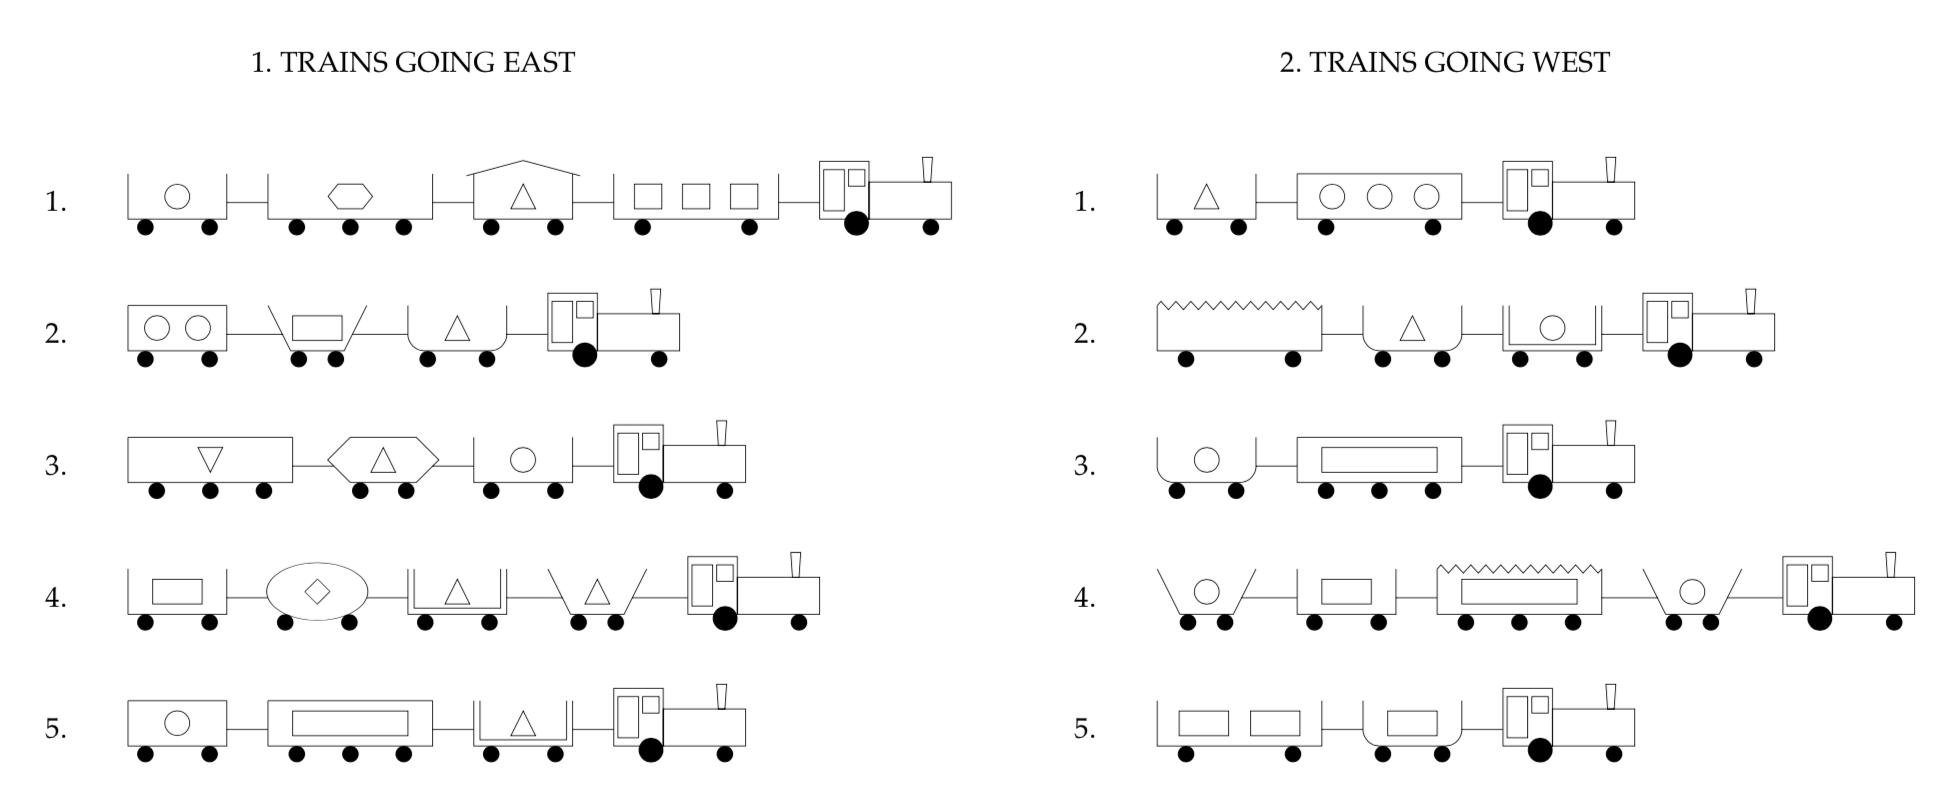
\includegraphics[width=\textwidth]{figs/trains}
\caption{Trains data set as introduced by Michalski.}
\end{figure}

The example of feature terms presented bellow is taken from the journal paper \textit{Similarity Measures over Refinement Graphs}  \cite{}. Consider the apparently simple Trains data set shown in Figure \ref{fig:TrainGraphic}, introduced by Michalski \cite{}: the original task is to learn the rule that discriminates east-bound from west-bound trains. If we were to represent such data set using a feature vector, we would need to define features for each one of the cars of a train (size, shape, load, and number of wheels), and determine beforehand a maximum number of cars per train (since feature vector representations have a fixed number of features).

Notice, however, that not all the trains have the same number of cars, and that, in principle, a train may have an unbounded number of cars. Thus, it is difficult to represent this data using a feature vector without losing information. Using a relational representation, we can just represent each car as a term, and define that a train is a set of cars, without restricting the number of cars of the train or the load each train is carrying.

\begin{figure}\label{fig:TrainFT}
\centering
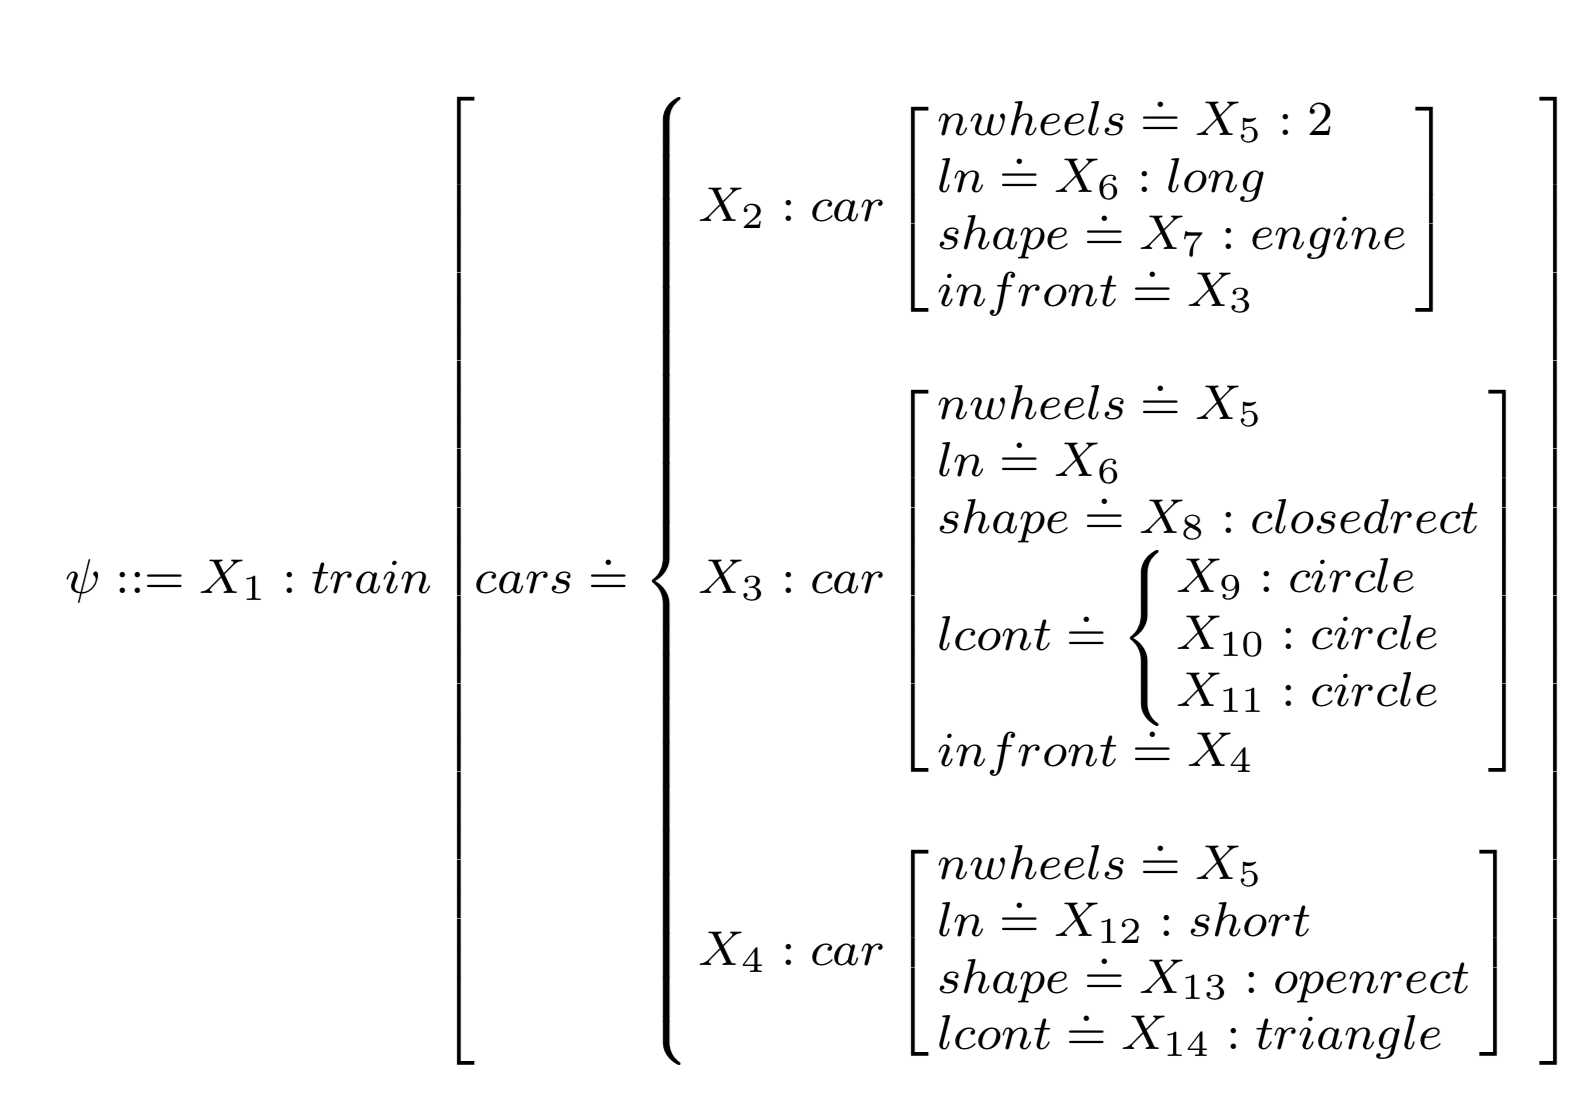
\includegraphics[scale = 0.4]{figs/trains3}
\caption{First west-bound train from Figure \ref{fig:TrainGraphic} represented in term notation.}
\end{figure}

On the other hand, Figure \ref{fig:TrainFT} represents the first west-bound train from Figure \ref{fig:TrainGraphic} using the feature term notation. We can see that the term is composed of 14 variables. The term contains two set- valued features (indicated by a curly bracket): in the feature cars of variable $X1$, and in the feature \emph{lcont} of variable $X3$. Finally, we can also see that there are several variable equalities in this term. Since the value of the feature \emph{infront} of variable $X2$ is the already defined variable $X3$, we note $X2.infront \doteq X3$, and also $X3.infront \doteq X4$. Additionally, the number of wheels in all the cars is the same, and the length of the first two cars is also the same.

The basic operation between feature terms is \emph{subsumption}: we will use $\psi_{1} \sqsubseteq \psi_{2}$ to express that a term $\psi_{1}$ subsumes another term $\psi_{2}$ – that is to say $\psi_{1}$ is more general (or equal) than $\psi_{2}$. Another interpretation of subsumption is that of an “informational content” order: $\psi_{1} \sqsubseteq \psi_{2}$ means that all the information in $\psi_{1}$ (all that is true for $\psi_{1}$) is also contained in $\psi_{2}$ (is also true for $\psi_{2}$)\footnote{In our work, we use the definition of subsumption introduced in \cite{} which has a slightly different definition than the traditional $\theta$-$subsumption$. Specifically, the difference is that we introduce the constraint that all the elements in a set have to be different.}.

\section{Concepts and Contrast Sets}\label{sec:Formalism}

\subsection{Semiotic Elements}\label{sec:SemEl}

The semiotic element are the components of concepts and containers. The different elements that an agent has perceived in its environment are called \emph{examples}. For example, a specific bird is an example of \emph{birds} or \emph{animals}. Birds and animals are two \emph{domains} in which we find birds. Domain is used here as a short for application domain.  Each example is identified by an index $i$ and noted $e_{i}$. Unless specified otherwise, agents are representing examples using a feature-term. A subset of a domain is a \emph{context}, the examples from the domain that a given agent has knowledge of, which we define in Definition \ref{def:Context}.

\begin{restatable}[Context]{df}{context}
\label{def:Context}
A context $U = \{ e_{1} \ldots e_{n} \}$ is a set of examples that covers a large part of a domain. 
\end{restatable}
A context needs to have enough examples to be partitioned into several non-empty sets.

An agent can classify the examples of a context into sets of examples called \emph{extensional definitions}. An extensional definition is associated to a specific category of the domain: for instance, the set of all birds of pray in a zoo can be an extensional definition for \emph{bird of prey} in the context of the zoo's aviary, for the domain of birds. Definition \ref{def:ExtD} formalizes this.

\begin{restatable}[Extensional Definition]{df}{extensional}
\label{def:ExtD}
An extensional definition is a non-empty subset of a context: $E_{i} \subset U$ and $E_{i} \neq \emptyset$. Extensional definitions are semiotic elements.
\end{restatable}

Some examples share similar features, and therefore can be generalized. A set of generalizations that generalize all the examples from an extensional definition is called an \emph{intensional definition} (see Def.\ref{def:IntD}). When the examples are represented as feature terms, the generalizations are also represented as feature terms that subsume sets of examples.

\begin{restatable}[Intensional Definition]{df}{intensional}
\label{def:IntD}
Let $X \subset U$ be a subset of examples of a context $U$, an intensional definition of $X$ is a set of generalizations $I_{i} = \{ g_{1}, \ldots , g_{n} \}$ such that $\forall e \in X, \exists g \in I_{i}$ such that $g \sqsubseteq e$, $\forall g \in I_{i}, \exists e \in X$ such that $g \sqsubseteq e$, and $\forall e' \in U-X, \nexists g \in I_{i}$ such that $g \sqsubseteq e'$. If an example $e$ is subsumed by a generalization from $I_{i}$, we note $I_{i} \sqsubseteq e$. Finally, we define as $X_{i} = \{ e \in U | I \sqsubseteq e \}$ the set of examples from $U$ that are subsumed by $I$.
\end{restatable}

When two agents are communicating, they are using \emph{signs} (see Def.\ref{def:Sign}). Signs are used to represent the labels of classes of examples. The knowledge representations that the agents use when they exchange examples or generalizations, feature terms for instance, are considered as represented by a system of signs -- even if it is not explicitly detailed. Notice that there is no constraint on the sign, therefore the choice of a sign for a concept is arbitrary. The arbitrariness of the sign means that all of those signs are \emph{symbols} from a semiotic point of view.

\begin{restatable}[Sign]{df}{sign}
\label{def:Sign}
A sign $s_{i}$ is a string of characters. Signs are semiotic elements.
\end{restatable}

The intensional, extensional definitions and the sign are the three primary semiotic elements. The relation between one sign, one intensional definition and one extensional definition is a \emph{concept}. The concepts bind the ability to partition a context (extensional and intensional definitions) to the ability to express this partition through communication (intensional definitions and signs). Concepts are also the last type of semiotic elements. The notion of concept is defined in Definition \ref{def:Con}.

\begin{restatable}[Concept]{df}{concept}
\label{def:Con}
A concept $C_{i} = (s_{i}, I_{i}, E_{i})$ is a triadic relation between a sign, an intensional definition and an extensional definition. Given a context $U$ and $X_{i} = \{ e \in U | I_{i} \sqsubseteq e \}$, the relation should verify that $E_{i} = X_{i}$. We note $I_{i} \sqsubseteq E_{i}$ the fact that $\forall e \in E_{i}$, $I_{i} \sqsubseteq e$. If the concept $C_{i}$ belongs to an Agent $A_{k}$, we note it $C_{i}^{k}$. Given an example $e$, if $I_{i} \sqsubseteq e$, we note $C_{i} \sqsubseteq e$. Concepts are semiotic elements.
\end{restatable}

When the context allows no confusion, we may simply write $s_{i}, I_{i}, E_{i}$ with the sub-index $i$ indicating the concept $C_{i}$ to which they belong. Otherwise, we will use the notation presented in Definition \ref{def:BFunctions} to refer to the specific constituents of a concept $C_{i}$.

\begin{restatable}[Concept Constituents]{df}{bFunctions}
\label{def:BFunctions}
For any concept $C_{i} = (s_{i}, I_{i}, E_{i})$

\begin{enumerate}
\item $s(C_{i}) = s_{i}$
\item $I(C_{i}) = I_{i}$
\item $E(C_{i}) = E_{i}$
\end{enumerate}

\end{restatable}

A same concept can be instantiated multiple times. For this reason, each concept $C_{i}$ has an identifier $id_{i}$. Two instances of concepts that share their identifier are supposed to be instances of a same concept. The identifier of a concept $C$ can also be noted $id(C_{i})$. One agent is not suppose to have more than one instance of a concept, and therefore cannot have two concepts sharing the same identifier.

%a group of semiotic elements are presented together in the text with the same index $i$, they are expected to be related to the same concept $C_{i}$.

\subsection{Containers And Contrast Sets}
\label{sec:Containers}

The agents are classifying the examples of their context. Each concept of an agent corresponds to a class, and the entire classification corresponds to a container. A container is the relation between a set of concepts and the context that this set of concepts is aiming to classify on, relation defined in Definition \ref{def:Cont}. There are two types of container: \emph{hypotheses} (see Def.\ref{def:Hyp}) and \emph{contrast sets} (see Def.\ref{def:Cset}). Hypotheses are not partitioning their context, while Contrast sets do.

\begin{restatable}[Container]{df}{container}
\label{def:Cont}
A container $Q = (U_{Q}, S_{Q})$ is a pair composed of a context $U_{Q}$ and a set of concepts $S_{Q} = \{ C_{1}, \ldots ,C_{n} \}$. The notation $C_i \in Q$ means that the concept $C_i$ belongs to the set of concepts $S_{Q}$, implying that $\forall C_{i} \in S_{Q}, E(C_i) \subset U_{Q}$.
\end{restatable}

Contrast sets are a type of container where the extensional definitions of the concepts are a partition of the context. Contrast sets are defined as follow:

\begin{restatable}[Contrast Set]{df}{contrastSet}
\label{def:Cset}
A contrast set $K = (U_{K}, \{ C_{1}, \ldots ,C_{n} \})$ is a container where the set of the extensional definitions $\{E(C_{1}), ... , E(C_{n})\}$ is a partition of the context $U_{K}$. This is noted as $\Pi(U_{K})= E(C_{1}), \ldots , E(C_{n})$. Moreover, the signs of the concepts must be different: $\forall C_{i},C_{j} \in K$, $i \neq j \Rightarrow s(C_{i}) \neq s(C_{j})$.
\end{restatable}

Recall that a partition of a set $S$ is a set of nonempty subsets of $S$ such that every element $e \in S$ is in exactly one of these subsets.

Hypotheses, as contrast sets, do not have more than one concept with the same size. However, unlike contrast sets, the extensional definitions of their concepts can have any relations as long as they remain compliant with the definition of containers.

\begin{restatable}[Hypothesis]{df}{hypothesis}
\label{def:Hyp}
A hypothesis $H = (U_{H}, \{ C_{1}, \ldots ,C_{n} \} )$ is a container where the signs of the concepts are different: $\forall C_{i},C_{j} \in H$, $i \neq j \Rightarrow s(C_{i}) \neq s(C_{j})$.
\end{restatable}

The agents are using contrast sets to know which sign to use in order to refer to one example from a domain. Hypotheses are used by agents to build a copy of other agents contrast sets with their own context in order to try to understand the point of view of other agents.

Concepts can be noted alternatively by using their signs or their identifiers. A concept from a contrast set or a hypothesis can be noted by using its sign and container, as two concepts from a same contrast set or hypothesis cannot share the same sign. Identifiers can be used to find a concept from any container of an agent, as an agent cannot have two concepts with the same identifier. This notation is useful to refer to a concept as a container's constituent, and is presented in Definition \ref{def:bFunctionsCtn} below:

\begin{restatable}[Container Constituent]{df}{bFunctionsCtn}
\label{def:bFunctionsCtn}
Let $A_{1}$ be an agent with $n$ containers $Q_{1} = \{S_{1}, U_{1} \},$ $\ldots,$ $Q_{n} = \{ S_{n}, U_{n}\}$ and $C_{i}$ a concept such that $C_{i} \in S_{i}$. If $s = s(C_{i})$ and $i = i(C_{i})$, therefore:

\begin{center}
    $C_{i} = C(s, Q_{i}) = C(i,A_{1})$.
\end{center}

\end{restatable}

\section{Agents}\label{sec:SemAg}

\paragraph{Knowledge}

Our approach focuses on pairs of agents that communicate together. Each agent is able to represent its knowledge with semiotic elements arranged in concepts, which are themselves arranged in containers. This allows the agents to have a partition of their contexts (the extensional definitions), a set of symbols to communicate over the examples of this partition (the signs) and generalizations to either incorporate new examples to their partition or access the reflexive function of language and address the meaning of their concepts in their communications with the other agent.

The two agents are numbered, called $A_{1}$ and $A_{2}$. Any agent can be referred as $A_{k}$, and in this case the other agent is referred as $A_{-k}$. An agent $A_{k}$ has knowledge over three containers: two contrast sets and one hypothesis. Among these two contrast sets, we distinguish the initial contrast set $K^{0}_{k}$ of an agent from the contrast set in use to communicate with the other agent $K_{k}$, called the \emph{current} contrast set. When an agent $A_{k}$ has a concept $C$ in its current contrast set, we say that $A_{k}$ \emph{knows} $C$.

The hypothesis $H_{k}$ of $A_{k}$ shares its context with $K$. $H_{k}$ is used to store the information that $A_{k}$ has on the other agent's concepts. As mentioned in Section \ref{sec:Containers}, hypotheses are used by agents to build a copy of other agents contrast sets with their own context in order to try to understand the point of view of other agents.

In general, any container $Q$ attached to an agent $A_{k}$ will be noted $Q_{k}$ while its context will be noted $U_{k}$ (see Section \ref{sec:SemEl}). A semiotic element $x$ attached to $A_{k}$ will be noted $x^{k}$.

\paragraph{Messages}

An agent can exchange information with the other agent using messages. A message $M(x_1, \ldots, x_n)$ contains $n$ semiotic elements. The letter $M$ is a place-holder for a \emph{performative}, that helps the agent that receives the message to understand what it is supposed to do with it. For instance, an agent receiving a message \emph{addExamples($e_1,e_2,e_3$)} knows that the other agent wants it to add the examples $e_1$, $e_2$ and $e_3$ to its contrast set's context.

By convention, when an agent $A_{k}$ wants to refer to two concepts in a message, one concept $C_{i}$ from its contrast set $K_{k}$ and another concept $C_{j}$ from the other agent's contrast set $A_{-k}$, $A_{k}$ starts its message with two signs: $s(C_{i})$ first and $s(C_{j})$ in second.

\paragraph{Functions}

The central function of an agent is to name an example when one is presented to it. In order to name an example $e$, an agent $A_{k}$ searches in its \emph{current} (not initial) contrast set $K_{k} = \{ U_{k}, S_{k} \}$ for the set of signs $N(A_{k},e) = \{ s(C) | C \in S_k \wedge I(C) \sqsubseteq e\}$ from the concepts of $S_{k}$ that are subsuming $e$. $A_{k}$ names the example $e$ with $N_{k}(e)$.

An agent has also access to various other functions that allow it to organize its contrast set and argue about it with another agent. These functions are presented later in detail in \ref{sec:AgentModel}.

\paragraph{Synchronization}

In order to have a synchronized communication, two agents are using a token when they communicate together. There is only one token in a communication between two agents. When an agent receives the token, the agent can act, using one or more of its functions. Once it is done with its actions, the agent passes the token to the other agent and waits until it receives the token back. The time lapse between the moment one agent receives the token and gives it back is called a \emph{turn}. The time lapse between two consecutive moments when one agent gets the token is called a \emph{round}.

\paragraph{States}

An agent's state determines which actions the agent will use during its turn. The next action that an agent takes during its turn is to pass the token to the other agent, regardless of the state, at the exception of the state where the agent stops the conversation. The second to last action that an agent takes during its turn is to select the state of its next turn. States are described later in Section \ref{sec:ArgSteps}.

\section{Relations between Concepts}

% The idea to map concepts

\subsection{Adjunct Sets and Relations}\label{sec:Adj&Relations}

\subsubsection{Adjunct Sets}\label{sec:Adj}

% How to map concepts
We saw in Section \ref{sec:SemAg} how the agents can name examples. For a given concept $C$ and a given example $e$ we can tell if an agent $A_{k}$, that has $C$ in the set of concepts of its current contrast set, has $s(C)$ in the set of signs $N_{k}(e)$ used to name $e$. In order to do so, we just need to verify that $I(C) \sqsubseteq e$: if this is the case, then $e \in N_{k}(e)$. Otherwise, $e \not \in N_{k}(e)$. If an agent $A_{k}$ returns $N_{k}(e)$ with a sign $s \in N_{k}(e)$ while naming an example $e$, we say that $A_{k}$ named $e$ with $s$.

We want to represent, for a given context $U$ and a given concept $C$, which examples from $U$ would be named $s(C)$ by an agent that has $C$ in its current contrast set. This brings us the notion of adjunct set defined below:

\begin{restatable}[Adjunct Set of a Concept]{df}{adjC}
\label{def:AdjC}
The adjunct set of a concept $C$ in the context $U$ is  $Adj(C,U) = \{ e \in U | I(C) \sqsubseteq e \}$. 
\end{restatable}

As we can see in Definition \ref{def:AdjC}, the adjunct set of a concept is independent of the sign or extensional definition of this concept. Indeed, only the intensional definition is needed to compute the adjunct set. Therefore, we can define the adjunct set of any set of generalizations as:

\begin{restatable}[Adjunct Set of an Intensional Definition]{df}{adjI}
\label{def:AdjI}
The adjunct set of an intensional definition $I$ in the context $U$ is  $Adj(I,U) = \{ e \in U | I \sqsubseteq e \}$. 
\end{restatable}

Both adjunct sets and extensional definitions are sets of examples and subsets of contexts. However, they are different because  extensional definitions are conceived as semiotic elements, while adjunct sets are an auxiliary notion conceived to compare concepts. An important property of adjunct set is that they are possible to link them to extensional definitions through the use of Property \ref{pp:Ext&Adj}.

\begin{restatable}[Extensional Definitions and Adjunct Set]{pp}{Ext&Adj}
\label{pp:Ext&Adj}

Let $C$ be a concept in the context $U$, such that $C = (s,I,J)$. If $C = (s,I,E)$ is a concept in the context $U$, therefore $E = Adj(C,U)$.

\end{restatable}

\begin{proof}
Let $C$ be a concept in the context $U$, such that $C = (s,I,J)$.
According to Definition \ref{def:Con}, $E = \{ e \in U | I \sqsubseteq e \}$.
According to Definition \ref{def:AdjC}, $Adj(C,U) = \{ e \in U | I \sqsubseteq e \}$.
Therefore, $E = Adj(C,U)$.
\end{proof}

\subsubsection{Pairing Partial Sets}\label{sec:PPSet}

The notion of adjunct set allows us to compare concepts. With the adjunct sets of any pair of concepts $C_{i}$ and $C_{j}$, it is possible to say for a given context $U$ which examples from $U$ would be named $s(C_{i})$ and not $s(C_{j})$, which examples from $U$ would be named $s(C_{j})$ and not $s(C_{i})$, and which examples from $U$ would be named both $s(C_{i})$ and $s(C_{j})$ by an agent that knows both concepts. In order to do so, we introduce the notion of pairing partial set. the three pairing partial sets represent the set relation between two adjunct sets from a same context. The notion of partial set is defined below:


\begin{restatable}[Pairing Partial Sets]{df}{pSet}
\label{def:PSet}
We define three  sets that characterize any pair of concepts $C_{i}$ and $C_{j}$: $U_{i,\overbar{j}}$, $U_{i,j}$ and $U_{\overbar{i},j}$. Theses three sets, called the pairing pairing partial sets, are defined as follows:
\begin{enumerate}
\item $U_{i,\overbar{j}} = Adj(C_{i}, U) - Adj(C_{j}, U)$
\item $U_{i,j} = Adj(C_{i}, U) \cap Adj(C_{j}, U)$
\item $U_{\overbar{i},j} = Adj(C_{i}, U) - Adj(C_{j}, U)$
\end{enumerate}
\end{restatable}

Let $A_{k}$ be an agent that knows both $C_{i}$ and $C_{j}$: while $A_{k}$ would name $s(C_{i})$ but not $s(C_{j})$ the examples from $U_{i,\overbar{j}}$, $s(C_{j})$ but not $s(C_{i})$ the examples from $U_{i,\overbar{j}}$ and both $s(C_{i})$ and $C_{j}$ the examples from $U_{i,j}$.

\subsubsection{Pairing Relations}\label{sec:Relations}

In order to represent the information that is given by the partial sets, we now introduce the notion of r-triplet. A r-triplet is a mathematical representation of the three partial sets of a given pair of concepts for a given context. This mathematical representation is a triplet of bits, each bit representing whether or not a given pairing partial set is empty. 

\begin{restatable}[R-Triplet Function]{df}{rTriplet}
\label{def:RTriplet}
The r-triplet function $r: \mathbb{X} \times \mathbb{X} \times \mathbb{U} \rightarrow  \{0, 1\}^{3}$, with $\mathbb{X}$ the domain of semiotic elements and $\mathbb{U}$ the domain of all possible contexts, is a function that for each pair of concepts $C_{i}$,$C_{j}$ and for a given context $U$ yields a triplet $(b_{-1},b_{0},b_{1})$ (called r-triplet) determined as follows:

\begin{enumerate}
\item $b_{-1} = \left\{
	\begin{array}{ll}
		0  & \mbox{if } U_{C_i,\overbar{C}_j} = \emptyset \\
		1 & \mbox{otherwise}
	\end{array}
\right.$
\item $b_{0} = \left\{
	\begin{array}{ll}
		0  & \mbox{if } U_{C_i,C_j} = \emptyset \\
		1 & \mbox{otherwise}
	\end{array}
\right.$
\item $b_{1} = \left\{
	\begin{array}{ll}
		0  & \mbox{if } U_{\overbar{C}_i,C_j} = \emptyset \\
		1 & \mbox{otherwsise}
	\end{array}
\right.$
\end{enumerate}
\end{restatable}

There are therefore $2^3 = 8$ possible r-triplets between two concepts $C_{i}$ and $C_{j}$ in the context $U$. The r-triplet gives the \emph{pairing relation} of $C_{i}$ and $C_{j}$ in $U$ accordingly to Definition \ref{def:Relation}:

\begin{restatable}[Pairing Relations]{df}{relation}
\label{def:Relation}
The pairing relations between a pair concepts $C_{i}$ and $C_{j}$ in a context $U$, represented with the operator $C_{i} r_{U} C_{j}$ where $r \in \{\equiv, \oslash, \odot, \otimes, \dagger, \circleddash \}$, are the following:

\begin{itemize}
\item if $r(C_i, C_j,U) = (0,1,0)$ they are in an \emph{equivalence} relation, noted $C_i \equiv_{U} C_j$ 
\item if $r(C_i, C_j, U) = (1,0,1)$ they are in is a \emph{disjunction} relation, noted $C_i \oslash_{U} C_j$ 
\item if $r(C_i, C_j, U) = (1,1,1)$ they are in is an \emph{overlap} relation, noted $C_i \otimes_{U} C_j$
\item if $r(C_i, C_j, U) = (1,1,0)$ or $r(C_i, C_j, U) = (0,1,1)$ they are in an inclusion relation, noted $C_i \odot_{U} C_j$
\item if $r(C_i, C_j, U) = (1,0,0)$ or $r(C_i, C_j, U) = (0,0,1)$ they are in a one-sided relation, noted $C_i \dagger_{U} C_j$.
\end{itemize}

Whenever $r(C_i, C_j, U) = (0,0,0)$, there is no pairing relation between the semiotic elements, which is noted $C_i \circleddash_{U} C_j$. 
\end{restatable}

According to Definition \ref{def:Relation}, there is no pairing relation when the adjunct sets of both $C_{i}$ and $C_{j}$ are empty. The pairing relation is one-sided when only one of the adjunct set is empty.

Each r-triplet has a corresponding \emph{reverse}. Let the reverse of a r-triplet be defined as follows: 
\begin{restatable}[R-Triplet Symmetry]{df}{rTSymmetry}
\label{def:RTSymmetry}
Let the matrix J be the exchange matrix of size $3 \times 3$:

\[
J = 
\begin{bmatrix}
    0 & 0 & 1\\
    0 & 1 & 0\\
    1 & 0 & 0\\
\end{bmatrix}
\]

The reverse of a r-triplet $R$ is the matrix product $RJ$. 

\end{restatable}

Let $C_{i}$ and $C_{j}$ be two concepts, and let $C_{i} r_{U} C_{j}$ be the pairing relation of $C_{i}$ with $C_{j}$ in $U$. Let $r(C_{i},C_{j}, U) = R$ and $r(C_{j}, C_{i}, U) = R'$. Since Definition \ref{def:PSet} shows that $R = R'J$ and $R' = RJ$, $R$ and $R'$ are the reverse of each other and therefore it is easy to see that each r-triplet gives the same pairing relation as its reverse r-triplet, $C_{i} r_{U} C_{j} = C_{j} r_{U} C_{i}$, therefore the operator $r_{U}$ from Definition \ref{def:Relation} is commutative.


\subsection{Overall Pairing Relations}\label{sec:Overall}

Let $A_{1}$ and $A_{2}$ be two agents, $A_{1}$ partitioning the context $U_{1}$ in the contrast set $K_{1} = \{ U_{1}, S_{1} \}$ and $A_{2}$ partitioning the context $U_{2}$ in the contrast set $K_{2} = \{ U_{2}, S_{2}\}$. If the agents want to compare two concepts $C_{i} \in S_{1}$ and $C_{j} \in S_{2}$, they can find the adjunct sets of both concepts, compute the corresponding pairing partial sets, use the function $r$ to find the r-triplet and deduce the pairing relation. However, the first element in the chain that allows the deduction of the pairing relation is the adjunct set. Since adjunct sets are context-dependent, the agents need to decide in which context they want to compare $C_{i}$ and $C_{j}$.

In an experimental set-up, there are three main contexts that are of interest. The two first context are $U_{1}$ and $U_{2}$, that are referred as the \emph{local} contexts, and the last one is the \emph{overall} context $U_{1} \cup U_{2}$ presented in Definition \ref{def:OContext}. Since two pairing relations in different local contexts might be different, and since the overall context includes both $U_{1}$ and $U_{2}$, the agents can agree that the overall r-triplet $r(C_{I},C_{J},U_{O})$ is obtained from more information than they currently dispose to compute their local r-triplets and therefore should supplant their local r-triplets. $C_{i}$ and $C_{j}$ in the overall context.

\begin{restatable}[Overall Context]{df}{overallContext}
\label{def:OContext}
The overall context $U_O = U_1 \cup U_2$ of two containers $Q_{1} = \{U_{1}, S_{1}\}$ and $Q_{2} = \{U_{2}, S_{2}\}$ is the union of their contexts $U_1$ and $U_2$.
\end{restatable}

In order to find an adjunct set $Adj(C, U_{O})$, the agents can exchange their respective adjunct sets $Adj(C, U_{1})$ and $Adj(C, U_{2})$ since $Adj(C, U_{O}) = Adj(C, U_{1}) \cup Adj(C, U_{2})$. However, this solution requires for the agents to exchange the adjunct sets. Since the adjunct sets can contain many examples, this represents a heavy transfer and is not the privileged solution. The agents have another solution, that allows them to find the pairing relation between $C_{i}$ and $C_{j}$ with far less data exchanged.

Computing the local r-triplet $r(C_{i}, C_{j}, U_{1})$ and $r(C_{i}, C_{j}, U_{2})$ only requires from the agents to transfer the intensional definitions $I_{i}$ and $I_{j}$, since with these two intensional definitions any agent $A_{k}$ can compute the adjunct set $Adj(C_{i}, C_{j}, U_{k})$ (see Definition \ref{def:AdjC}). By exchanging their local r-triplets, the agents can finally infer the \emph{overall} pairing relation using Theorem \ref{thm:Overall}.
 
\begin{restatable}[Expression of Overall Pairing Relation]{thm}{Overall}\label{thm:Overall}
Let $A_{1}$ and $A_{2}$ be two  agents, $A_{1}$ partitioning the context $U_{1}$ in the contrast set $K_{1} = \{ U_{1}, S_{1} \}$ and $A_{2}$ partitioning the context $U_{2}$ in the contrast set $K_{2} = \{ U_{2}, S_{2}\}$. Let $C_{i} \in S_{1}$ and $C_{j} \in S_{2}$ be two concepts, and
\begin{itemize}
%\item the two local triplets:
%\begin{itemize}
\item let $r(C_{i},C_{j},U_{1}) = (b_{-1}, b_{0}, b_{1})$ be the local triplet of $A_{1}$
\item let $r(C_{i},C_{j},U_{2}) = (b'_{-1}, b'_{0}, b'_{1})$ be the local triplet of $A_{2}$
%\end{itemize}
\item  let $r(C_{i}, C_{j}, U_{O}) = (b''_{-1}, b''_{0}, b''_{1})$ be the overall triplet $A_{1}$ and $A_{2}$
\end{itemize}
then, for all $n \in \{-1, 0, 1\}$, the element of the overall triplet $b_{n}''=0 \Leftrightarrow b_{n} = 0 \wedge b_{n}' = 0$, and otherwise $b_{n}''=1$.
\end{restatable}

\begin{proof}
See Appendix \ref{proof:ThmOverall}.
\end{proof}

Theorem \ref{thm:Overall} results in four common and remarkable cases of local pairing relations for which the overall relation can be inferred just by transferring the two local pairing relations an not the local r-triplets. These four cases are listed below in Theorem \ref{thm:ROverall}:

\begin{figure}[t]\label{fig:VennCases}
\centering
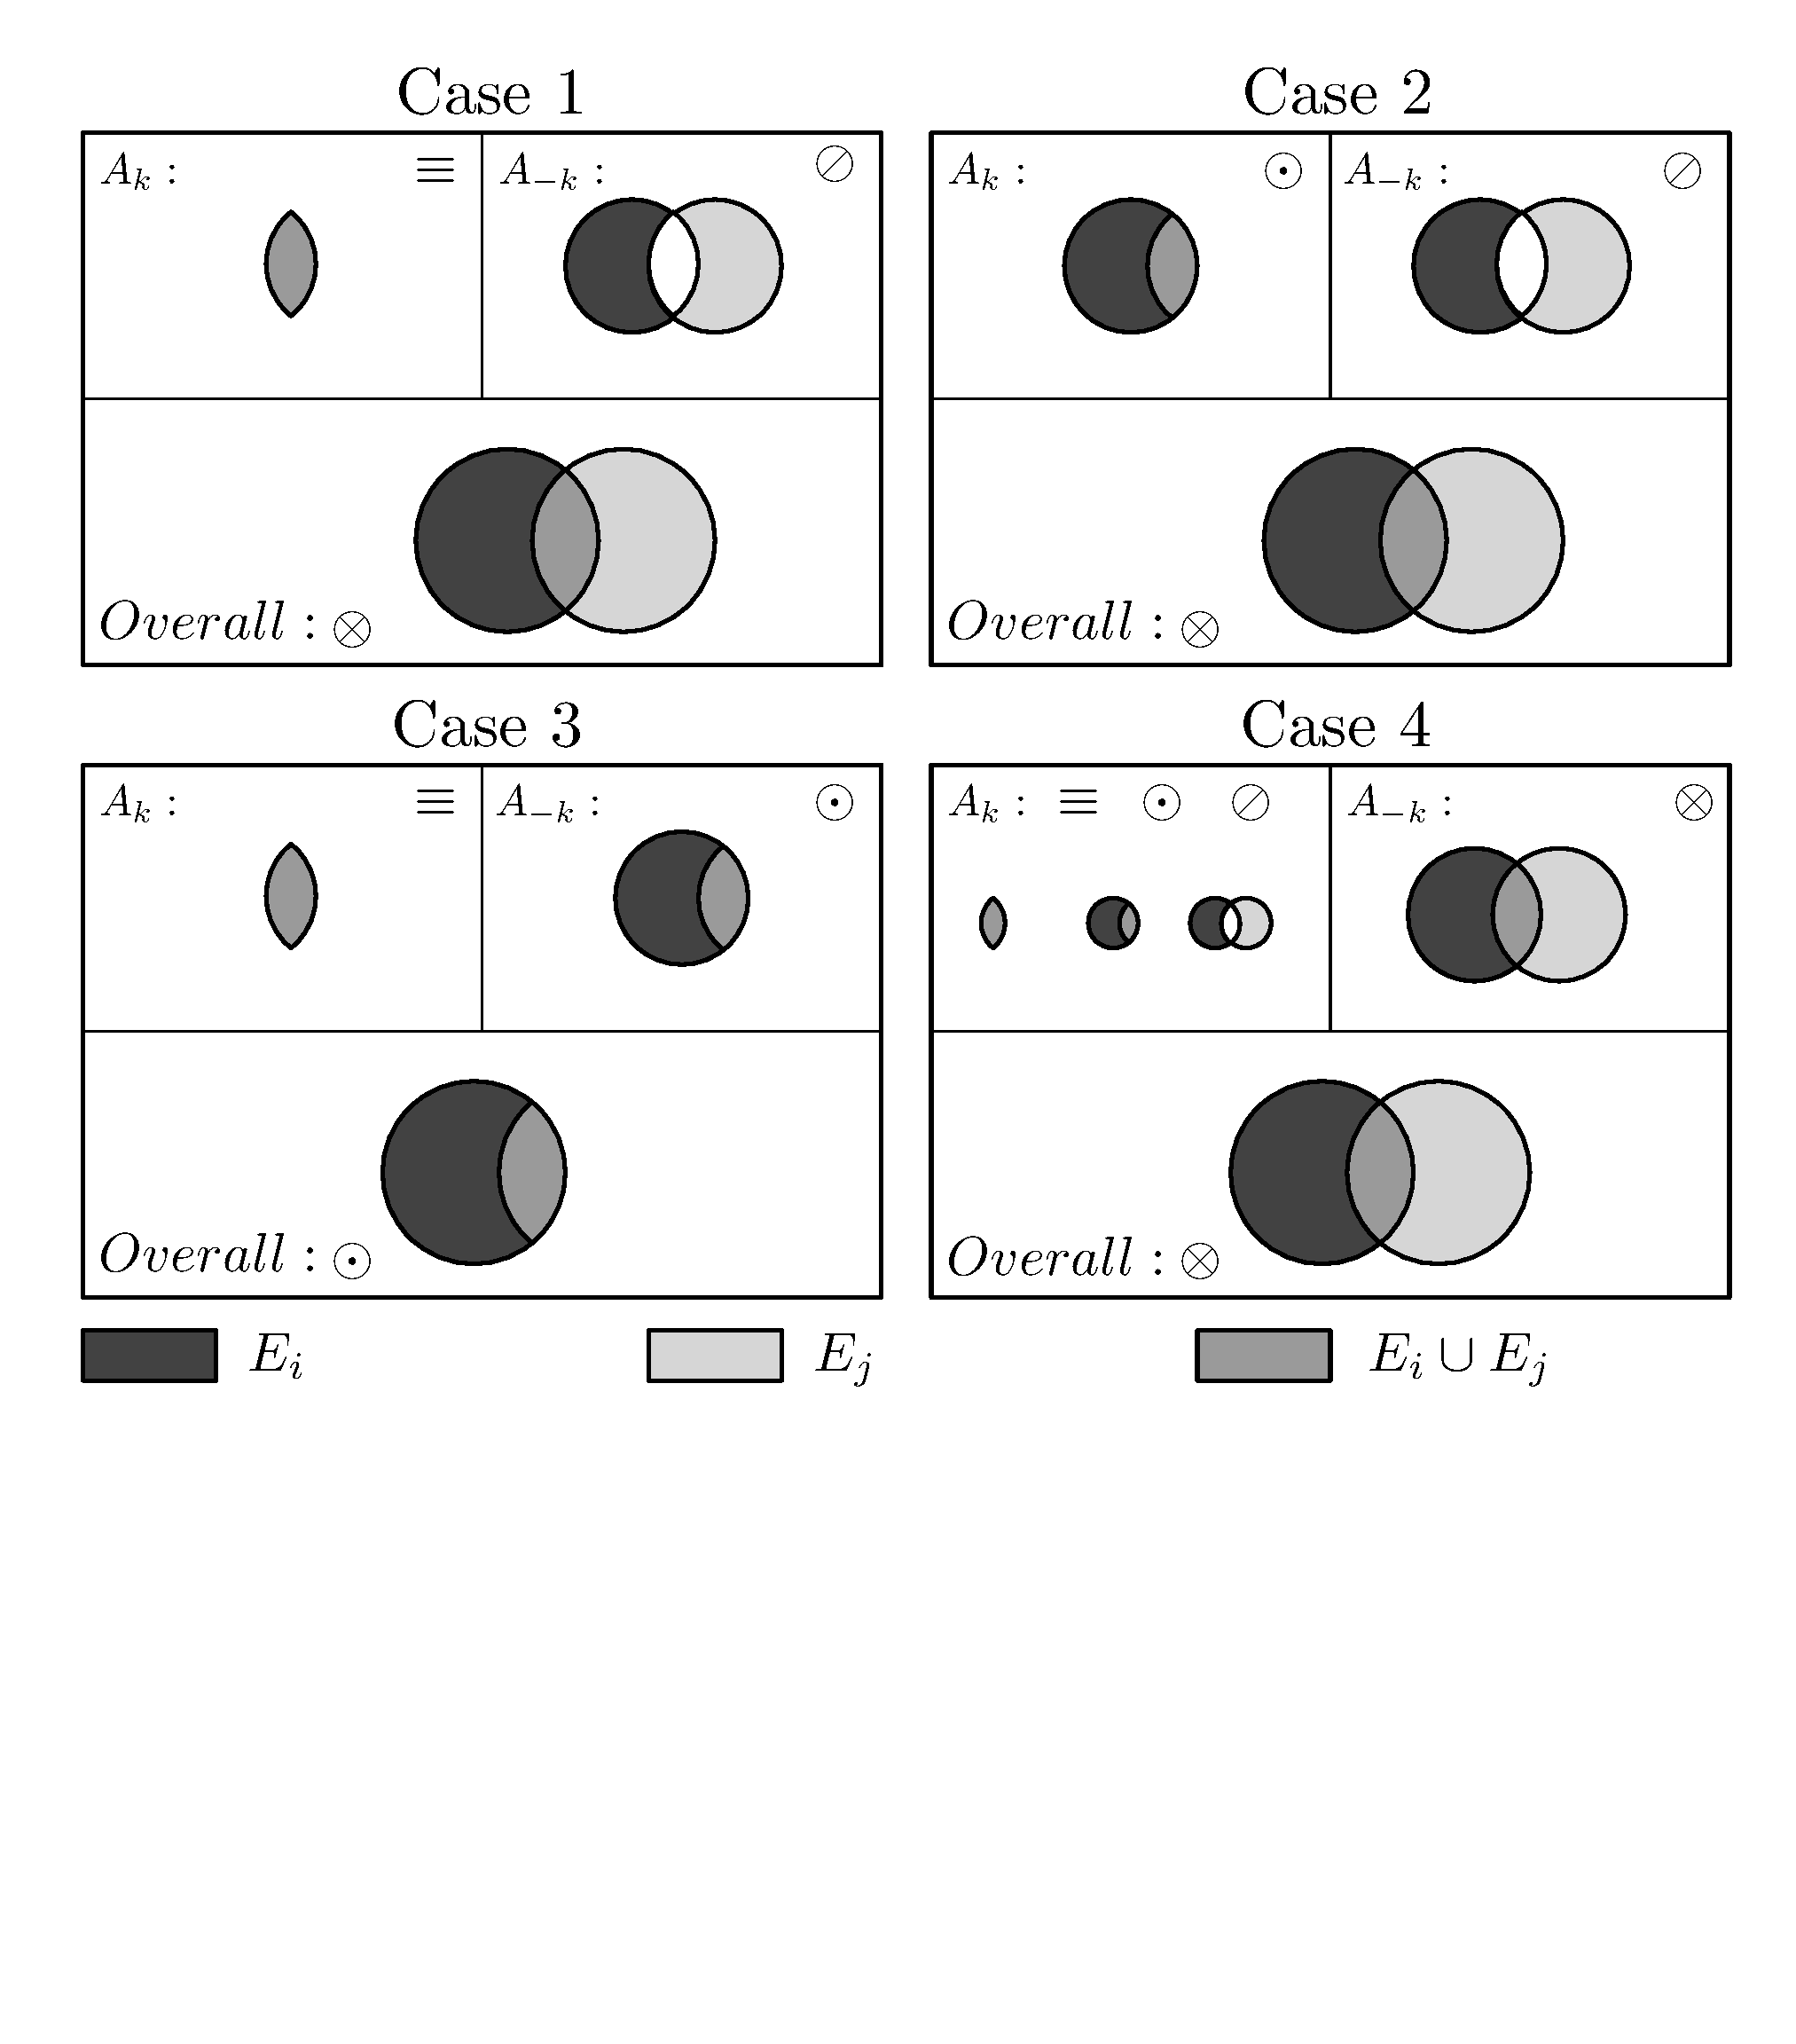
\includegraphics[scale=0.35]{figs/cases.pdf}
\caption{Venn diagrams illustrating of the four cases where it is possible to infer an overall relations' type from its two corresponding local relations' types.}
\end{figure}

\begin{restatable}[Overall Pairing Relation of Different Local Relations]{thm}{rOverall}
\label{thm:ROverall}

Let $A_{1}$ and $A_{2}$ be two agents, $A_{1}$ partitioning the context $U_{1}$ in the contrast set $K_{1} = \{ U_{1}, S_{1} \}$ and $A_{2}$ partitioning the context $U_{2}$ in the contrast set $K_{2} = \{ U_{2}, S_{2}\}$. Let $C_{i}$ and $C_{j}$ be two concepts such that $C_{i} \in S_{1}$ and $C_{j} \in S_{2}$. Let $C_{i} r_{U1} C_{j}$ be the local pairing relation of the agent $A_{1}$ and $C_{i} r_{U2} C_{j}$ the local pairing relation of the agent $A_{2}$, if $C_{i} r_{O} C_{j}$ is the overall pairing relation of $A_{1}$ and $A_{2}$ between $C_{i}$ and $C_{j}$, then the following holds:

\begin{enumerate}
\item if $C_{i} \equiv_{U1} C_{j}$ and $C_{i} \oslash_{U2} C_{j}$, then $C_{i} \otimes_{O} C_{j}$ %\textbf{(case 1)}.
\item if $C_{i} \odot_{U1} C_{j}$ and $C_{i} \oslash_{U2} C_{j}$, then $C_{i} \otimes_{O} C_{j}$ %\textbf{(case 2)}.
\item if $C_{i} \equiv_{U1} C_{j}$ and $C_{i} \odot_{U2} C_{j}$, then $C_{i} \odot_{O} C_{j}$ %\textbf{(case 3)}.
\item if $C_{i} \equiv_{U1} C_{j}$, $C_{i} \odot_{U2} C_{j}$ or $C_{i} \oslash_{U1} C_{j}$ and $C_{i} \otimes_{U2} C_{j}$, then $C_{i} \otimes_{O} C_{j}$ %\textbf{(case 4)}.
\end{enumerate}

\end{restatable}

\begin{proof}
See Appendix \ref{ap:3}
\end{proof}

At last, since the r-triplets of the pairing relations of equivalence, disjunction and overlap are symmetrical (let $R$ be a r-triplet that corresponds to a relation equivalence, disjunction or overlap. We can observe in Definition \ref{def:Relation} that in these three cases, $R = RJ$), if two local pairing relations are both equivalences, disjunctions or overlaps then the overall pairing relation will be from the same type. For the remaining cases, the agents have no choice but to exchange their local r-triplets instead of their local pairing relations in order to infer the overall pairing relation.

\section{Agreement and Disagreement}\label{sec:AgreeDisagree}

\subsection{Mutual Intelligibility and Monotonicity}\label{sec:MutInt}

The argumentation on meaning revolves around mutual intelligibility. Mutual intelligibility is context dependent, and refers to a state of the multi-agent system where both agents are able to name every example from a given context with the same sign. Since the agents are not meant to go through an extensive naming game over an entire context outside of the experimental context of our thesis, mutual intelligibility refers also to a state where both agents agree that there is no example from a given context that they would -- to their knowledge -- name differently than the other agent.

The notion of mutual intelligibility is attached to two properties. First, both agents should partition the context of their mutual intelligibility into the same segregates, at least theoretically. Then, both agents should map these segregates to the same signs. Having these two properties, equal partition and equal sign-mapping for both agents, guarantees the mutual intelligibility between the agents over a given context. This notion of mutual intelligibility is formalized in Definition \ref{def:MIntel}.

\begin{restatable}[Mutual Intelligibility]{df}{mIntel}\label{def:MIntel}
Let $A_{1}$ and $A_{2}$ be two agents that have for respective contrast sets $K_{1} = (U_{1},S_{1})$ and $K_{2} = (U_{2},S_{2})$.  $A_{1}$ and $A_{2}$ have reached mutual intelligibility under the limits of a context $U$ whenever $\forall e \in U$, $!\exists C_{i} \in S_{1}$ and  $!\exists C_{j} \in S_{2}$ such that $C_{i} \sqsubseteq e$ and $C_{j} \sqsubseteq e$ and $s(C_{i}) = s(C_{j})$. 
\end{restatable}

Now that we stated multiple times that the ultimate goal of our agents is to reach mutual intelligibility and that we have formally defined this mutual intelligibility, we need to address the question of the mutual intelligibility's context. Since the mutual intelligibility is context dependant, the agents need know over which context they are trying to reach it in order to coordinate. We will assume that this context has examples from both agents, that are however not in both current contrast sets' context, which is the most complex possible scenario. In this scenario, each agent $A_{k}$ could send to the other agent $A_{-k}$ the set of the examples from $U_{k}$ that are not in $U_{-k}$. However, this requires for each agent $A_{k}$ to know which are these examples and thus have knowledge over $U_{-k}$.

Another solution that does not necessitate for $A_{k}$ to have knowledge over $U_{-k}$ is to know the pairing relations between the concepts that have examples in the context $U$ over which the mutual intelligibility is wished. Theorem \ref{thm:RMIntel} draws a direct correspondence between the definition of a mutual intelligibility over the context $U$ and the pairing relations between concepts in $U$. 

\begin{restatable}[Constraints on Relations for Mutual Intelligibility]{thm}{RMIntel}
\label{thm:RMIntel}
Let $A_{1}$ and $A_{2}$ be two agents with contrast sets $K_{1} = (U_{1},S_{1})$ and $K_{2} = (U_{2},S_{2})$. Let $U$ be a context such that $U \subseteq U_{O}$. We say that $A_{1}$ and $A_{2}$ have reached mutual intelligibility within the context $U$ according to Definition \ref{def:MIntel} if for each concept $C_{i} \in S_{1}$ whenever either:

\begin{itemize}
    \item[a.] $\forall C_{j} \in S_{2}, C_{i} \circleddash_{U} C_{j}$ 
\end{itemize}

holds, or (\textbf{exclusive or}) all of the following holds:

\begin{itemize}
    \item[b.] $!\exists C_{k} \in S_{2}$ such that $C_{i} \equiv_{U} C_{k}$
    \item[c.] \textbf{and} $\forall C_{j} \in S_{2}$, one of the two following holds:
    \begin{itemize}
    \item[$c1$.] $C_{i} \equiv_{U} C_{j}$
    \item[$c2$.] $C_{i} \oslash_{U} C_{j}$
    \end{itemize}
    \item[d.] \textbf{and} $ \forall C_{j} \in S_{2}$:
    \begin{itemize}
        \item[$d1$.] if $C_{i} \equiv_{U} C_{j}$ then $s(C_{i}) = s(C_{j})$
        \item[$d2$.] if $C_{i} \oslash_{U} C_{j}$ then $s(C_{i}) \neq s(C_{j})$
    \end{itemize}
\end{itemize}

\end{restatable}

\begin{proof}

\end{proof}

With Theorem \ref{thm:RMIntel} the agents can now infer a mutual intelligibility over the context $U$ from the overall pairing relations of the concepts involved in the context $U$. The agents can figure the overall pairing relations between concepts by exchanging r-triplets as explained in Section \ref{sec:Overall}. Therefore, the agents do not need to exchange examples in order to know if they have reached a mutual intelligibility over a context -- even if examples of this context are not shared by both agents.

While we repeatedly asserted that the aim of the argumentation between our two agents is to reach mutual intelligibility, the mutual intelligibility itself cannot be the only goal. We can intuitively think of two unsatisfying solutions that always guarantee a mutual intelligibility; the first one is having both agents' current contrast sets $K_{1} = \{U_{1}, S_{1} \}$ and $K_{2} = \{U_{2}, S_{2} \}$ with $S_{1} = \{ C_{i} \}$ and $S_{2} = \{ C_{j} \}$ such that $C_{i}$ and $C_{j}$ both have the same sign $s_{all}$ and an intensional definition that subsumes all possible examples. In a such scenario, any example would be immediately be named $s_{all}$ by both agents which is, by definition, a mutual intelligibility. The second scenario would be one agent $A_{1}$ copying the current contrast set $K_{2} = \{U_{2}, S_{2} \}$ of the other agent $A_{2}$. In this situation, the agents have the same contrast set $(K_{1} = K_{2})$ and therefore have reached mutual intelligibility over any context that is a subset of $U_{2}$.

These in these two scenarios, mutual intelligibility has been reached over large contexts. However, if we assume that the initial contrast sets of the agents are a classification that had a purpose, we wish to have any current contrast set also able to fit this purpose no matter no matter what it is. For this reason, the agents only have current contrast sets that are \emph{refinement} of their initial contrast set. By making sure that its new contrast sets are refinements of its initial one, an agent has the guarantee that two examples initially classified in different concept remains labelled as belonging to different classes. This monotonic evolution of contrast sets is formalized in Definition \ref{def:SCon}. 

\begin{restatable}[Monotonicity]{df}{sCon}
\label{def:SCon}
Let $A$ be an agent that has an initial contrast set $K^{0} = \{U_{0}, S_{0} \}$. If $A$ creates a new contrast set $K_{1} = \{U_{1}, S_{1} \}$ as its current contrast set, $A$'s contrast sets are monotone if $U_{0} \subseteq U_{1}$, and if for all pairs of examples $e_{1},e_{2} \in U_{0}$ and for every concept $C_{1} \in S_{1}$, there exists $C_{0} \in S_{0}$:

\begin{center}
$e_{1},e_{2} \in E(C_{1}) \Rightarrow e_{1},e_{2} \in E(C_{0})$
\end{center}

\end{restatable}

\subsection{Agreement over Meaning}\label{sec:Agree}

The mutual intelligibility and the monotonicity are the formalizations of the agents goal during the argumentation. In order to reach this goal, the agents need to be able to evaluate them and identify any eventual problem that would prevent the goal's realisation.

\subsubsection{Synchronic Agreement}\label{sec:SynAg}

The synchronic agreement is a state of one agent where this agent cannot find any overall pairing relation that would contradict the mutual intelligibility as defined in Theorem \ref{thm:RMIntel}. When both agents are in a state of synchronic agreement, we say that the agents have reached mutual intelligibility.

Unlike the mutual intelligibility, the synchronic agreement can be unilateral. This occurs when one agent has access to more overall relations than the other. In this case, the former agent can know about the situation of a pair of concepts that does not satisfy the criteria listed in Definition \ref{def:MIntel} as presented in Theorem \ref{thm:RMIntel}, while the latter agent ignores the situation of this pair of concepts.

\subsubsection{Diachronic Agreement}\label{sec:DiaAg}

The diachronic agreement is a state of one agent where this agent current contrast set is a refinement of this agent initial contrast set as defined in Definition \ref{def:SCon}. Unlike the synchronic agreement, the diachronic agreement is always verified. Since the monotonicity is a constraint put on the creation of new contrast sets, no current contrast set can be created in a non-monotonic way.

\subsection{Types of Disagreements}\label{sec:Disagree} 

\subsubsection{Synchronic Disagreements}\label{sec:SynD}

The Theorem \ref{thm:RMIntel} gives, for a list of pairs of concepts and a context, the pairing relations and the relations between the signs that the two concept of each pair should observe in order to have a mutual intelligibility between the agents. If one pair of concept does not observe these properties in the context of the expected mutual intelligibility, the agents do not have the mutual intelligibility. We call such a pair a synchronic \emph{disagreement}. The notion of synchronic disagreement is defined below:

\begin{restatable}[Synchronic Disagreement]{df}{synDg}
\label{def:SynDg}
Let $A_{1}$ and $A_{2}$ be two agents that have for respective contrast sets $K_{1} = (U_{1},S_{1})$ and $K_{2} = (U_{2},S_{2})$. Let $U$ be a context such that $U \subseteq U_{1} \cup U_{2}$. Let $C_{1}$ and $C_{2}$ be two concepts such that $C_{1} \in S_{1}$ and $C_{2} \in S_{2}$. $A_{1}$ and $A_{2}$ have a synchronic disagreement over $C_{1}$ and $C_{2}$ within context $U$ whenever one of the following conditions holds:

\begin{enumerate}
\item $C_{i} \odot_{U} C_{j}$
\item $C_{i} \otimes_{U} C_{j}$
\item $C_{i} \dagger_{U} C_{j}$
\item $C_{i} \equiv_{U} C_{j}$ and $s_{i} \neq s_{j}$
\item $C_{i} \oslash_{U} C_{j}$ and $s_{i} = s_{j}$
\end{enumerate}

or if there exists a concept $C_{k} \in S_{k}$ while there is no concept $C_{-k} \in S_{-k}$ such that $C_{k} r_{U} C_{-k}$.

\end{restatable}


These six conditions give rise to 6 types of disagreement, defined as follows:

\paragraph{Hypo-hypernymy Disagreement} If $C_{i} \odot_{U} C_{j}$, then one concept is the  hyponym of the  other (and the second concept is the hypernym of the first). More specifically, if $r(C_{i},C_{j},U) = (1,1,0)$ then $C_{i}$ is the \emph{hypernym} of $C_{j}$, while if $r(C_{i},C_{j},U) = (0,1,1)$ $C_{i}$ is the \emph{hyponym} of $C_{j}$. A hypo-hypernymy disagreement is expressed as $(s_{i},s_{j},C_{i} \odot_{U} C_{j})$.

\paragraph{Overlap Disagreement} If $C_{i} \otimes_{U} C_{j}$, the two concepts are said to overlap. An overlap disagreement is expressed as $(s_{i},s_{j},C_{i} \otimes_{U} C_{j})$.

\paragraph{Synonymy Disagreement} If $C_{i} \equiv_{U} C_{j}$ and $s_{i} \neq s_{j}$, we have two concepts that are equivalent but their corresponding signs are different (therefore they are synonyms). A synonymy disagreement is expressed as $(s_{i},s_{j},C_{i} \equiv_{U} C_{j})$.

\paragraph{Homonymy Disagreement} If $C_{i} \oslash_{U} C_{j}$ and $s_{i} = s_{j}$,  we have two concepts that are disjoint  but their corresponding signs are equal (therefore they are homonyms). A homonymy disagreement is expressed as $(s_{i}, s_{j},C_{i} \oslash_{U} C_{j})$.

\paragraph{Untranslatability Disagreement} If $C_{i} \not \equiv_{U} \bullet$, we have a concept $C_{i}$ that cannot found a concept $C_{j}$ such that $C_{i} \equiv_{U} C_{j}$. The symbol ``$\not \equiv$'' does not refer to a paring relation here, but to the absence of a pairing relation of equivalence. Moreover, the symbol ``$\bullet$'' does not represent a specific concept, but any concept from $S_{2}$.

Each of the five first disagreement types can be represented as a triplet $(s_{1}, s_{2}, r_{U})$ where $s_{1}$ and $s_{2}$ are the signs of the first and second concepts, and where $r_{U}$ their relation in the context of the expected mutual intelligibility. Since one type of disagreement corresponds to exactly one type of pairing relation, $r$ qualifies the type of disagreement as it already qualifies the type of pairing relation. The untranslatability disagreement is a special case, noted $(s_{1}, \bullet, \not \equiv_{U})$.

\paragraph{Indistinguishable Disagreement} If $C_{i} \dagger_{U} C_{j}$, or if $C_{i}$ and $C_{j}$ do not have a pairing relation, the two concepts are said to be indistinguishable. While this disagreement cannot appear with regular (Boolean) r-triplets, it appears when we later assume a degree of error that requires integer r-triplets in Section \ref{sec:DoGGenIdea}.

\subsubsection{Classification of Synchronic Disagreements}\label{sec:SynDclass}

Other than according to their types, the synchronic disagreements can be regrouped by families. Synchronic disagreements are regrouped in main families that will later determine the approach that our agents will display to solve them. There are four families of synchronic disagreements: \emph{self}-disagreements, \emph{semantic} disagreement, \emph{lexical} disagreements and \emph{untranslatable} disagreements.

\paragraph{Semantic Disagreement} The semantic disagreements are hypo/hypernymy, overlap and indistinguishable disagreements involving two concepts from different agents, that require the refinement of one or two of the agents' concept(s) in order to be solved. Semantic disagreements require either a specific argumentation on meaning in order to create new concepts that are hyponyms of the older ones that cause the disagreement, or the deletion of one of the two concepts in the case of the indistinguishable type of disagreements.

\paragraph{Lexical Disagreement} The lexical disagreements are synonymy and homonymy disagreements involving two concepts from different agents, that require a sign change for one or more of the agents' concepts. Lexical disagreements are solved through the creation of new signs, without modifying any other type of semiotic elements.

\paragraph{Self-Disagreement} The self-disagreements can be any type of disagreements. However, unlike other families, the self-disagreements involve two concepts that are from the same agent. Due to the fact that the two concepts belong to the same initial contrast-set, which is a partition of the agent's context, a self-disagreement cannot be anything else than an overlap disagreement. Unlike overlaps that belong to the semantic disagreements, the self-disagreements are solved through a process named "border-alignment" instead of creating a new concept.

\paragraph{Untranslatable Disagreements} The untranslatable disagreements regroup the disagreements of the eponymous type. With the self-disagreement, this is the only family that does not involve two concepts from different agents, although it is because it only involves one concept. An untranslatable disagreement is solved by creating an equivalent concept to the one involve in the disagreement, and adding it to the contrast-set that misses it.


\subsubsection{Diachronic Disagreements}\label{sec:DiaD}

As explained in Section \ref{sec:DiaAg}, there is no diachronic disagreement. The fact that an agent $A$ has knowledge over its initial contrast set allows $A$ to create new concepts for its current contrast set that are not violating the diachronic agreement. The fact that the monotonicity is defined on the context of the initial contrast set, that does not change through the argumentation, ensures that no diachronic disagreement can appear following the addition of a new example to the current contrast set's context.

\subsection{Connected Sets of Disagreements}
\label{sec:SystemDisagreement}

Our approach is centered on the ability to simplify a communication issue between two agents, involving multiple concepts, into a list of smaller disagreements that each involves only two concepts. At an intermediary level between the interconnected graph of pairing relations and the pairs of disagreement, we have connected sets of disagreements.

\begin{restatable}[Connected Sets of Disagreements]{df}{ConnectedDisagreement}
\label{df:ConDisagreement}

Let $D = d_{1}, \ldots, d_{n}$ be a set of synchronic disagreements in a context $U$. Let $D_{1}$ be a set of disagreement such that $D_{1} \subseteq D$. $D_{1}$ is a connected set of disagreement from $D$ if:

\begin{itemize}
    \item $\forall d_{x} \in D_{1}$ such that $d_{x} = (s_{1}, s_{2},C_{1} r_{U} C_{2})$, $\exists d_{y} \in D_{1}$ such that $d_{y} = (s_{1}', s_{2}',C_{1}' r_{U} C_{2}')$ and $C_{1} = C_{1}'$, $C_{1} = C_{2}'$, $C_{2} = C_{1}'$ or $C_{2} = C_{2}'$
    \item $\forall d_{x} \in D_{1}$ such that $d_{x} = (s_{1}, s_{2},C_{1} r_{U} C_{2})$, $\nexists d_{z} \in \{D - D_{1}\}$ such that $d_{z}= (s_{1}'', s_{2}'',C_{1}'' r_{U} C_{2}'')$ and $C_{1} = C_{1}''$, $C_{1} = C_{2}''$, $C_{2} = C_{1}''$ or $C_{2} = C_{2}''$
\end{itemize}

\end{restatable}

Intuitively, connected sets of disagreements are disjoint subsets of a general set of disagreements -- usually the set of all the synchronic disagreements between two agents -- that are clustered according to the concepts that are causing the disagreements within them.

\section{Complement to the Notation}\label{sec:FormRemarks}

\subsection{On Concepts Sharing Signs}\label{sec:SharingSigns}
The protocol that we presented in the past sections has been tested in experimental scenarios of increasing complexity. All the scenarios are based on a data set that has been modified in order to create controlled instances of disagreements. Since sometimes the concepts $C_{i}^{k}$ from $A_{k}.K$ and $C_{j}^{-k}$ from $A_{-k}.K$ will be in a situation where $i = j$. In this situation, the concept $C_{i}$ from $A_{K}$ and the concept $C_{j}$ from $A_{k}.H$ can be both noted $C_{i}^{k}$ or $C_{j}^{k}$. In order to remove this ambiguity, we will note $C_{j'}^{k}$ the concept that belongs to $A_{k}.H$. This way, the apostrophe marks the belonging to a hypothesis. In the situation where $i \neq j$, the absence of ambiguity allows us to not put the apostrophe.

\subsection{On Hyponyms and Hypernyms}\label{sec:OnHypoHyper}
During the previous sections, four notions from linguistics (hyponymy, hypernymy, synonymy and homonymy) have been used  to characterize the relation between two concepts.  We add now a fifth notion, the co-hyponymy. A set of concepts $C_{h_{1}}, \ldots , C_{h_{n}}$ are co-hyponyms of a common hypernym $C_{H}$ if the co-hyponyms' extensional definitions $E_{h_{1}}, \ldots , E_{h_{n}}$ are a partition  of the hypernym's extensional definition $E_{H}$. The correct syntax to express co-hyponymy is: $C_{h_{1}}$ is co-hyponym \emph{of} $C_{H}$ \emph{with} $C_{h_{2}}, \ldots , C_{h_{n}}$.

\begin{restatable}[Co-Hyponyms]{df}{coHypo}
\label{def:CoHypo}
Let $C_{H}$ be a concept, $C_{1}, \ldots, C_{n}$ be $n$ concepts with $n > 2$, and $U$ a context such that:

\begin{enumerate}
    \item $\forall x \in \{1, \ldots, n\}, Adj(C_{x},U) \subset Adj(C_{H},U)$
    \item $\forall x,y \in \{1, \ldots, n\}, C_{x} \odot_{U} C_{y}$
    \item $Adj(C_{1},U) \cup \ldots \cup Adj(C_{n},U) = Adj(C_{H},U)$
\end{enumerate}

then $C_{1}, \ldots, C_{n}$ are co-hyponyms of $C_{H}$

\end{restatable}

\subsection{Computing Multiple R-Triplets and Pairing Relations}\label{sec:MultipleRelations}

When an agent computes multiple r-triplet or pairing relations, we simplify the notation of the set of elements computed. Given two sets of concepts $S_{1} = \{C_{1,1}, \ldots, C_{1,m} \}$ and $S_{2} = \{C_{2,1}, \ldots, C_{2,n} \}$, the set of R-Triplets $T(S_{1} \times S_{2}, U)$ is equal to:

\begin{center}
    $\{ r(C_{1,1}, C_{2,1}, U)$, $\ldots$, $r(C_{1,1}, C_{2,n}, U)$,\\
    $\ldots$\\
    $r(C_{1,m}, C_{2,1}, U)$, $\ldots$, $r(C_{1,m}, C_{2,n}, U) \}$
\end{center}


and the set of pairing relations $R(S_{1} \times S_{2}, U)$ is equal to:

\begin{center}
    $\{ C_{1,1} r_{u} C_{2,1}$, $\ldots$, $C_{1,1} r_{u} C_{2,n}$,\\
    $\ldots$\\
    $C_{1,m} r_{u} C_{2,1}$, $\ldots$, $C_{1,m} r_{u} C_{2,n} \}$
\end{center}

\subsection{R-Triplets and Associated Pairing Partial Sets}

The presentation of r-triplets in Section \ref{sec:Relations} introduced how each value of a r-triplet figures the state of emptiness of a particular pairing partial set. Let $C_{i}$ and $C_{j}$ be two concepts, $U$ a context and $U_{-1}, U_{0}$ and $U_{1}$ three partial sets such that:

\begin{itemize}
    \item $U_{-1} = U_{C_{i},\overbar{C_{j}}}$,
    \item $U_{0} = U_{C_{i},C_{j}}$ and 
    \item $U_{1} = U_{\overbar{C_{i}},C_{j}}$.
\end{itemize}

Let \emph{bool(p)} be a function that takes a proposition $p$ as a parameter and returns 1 if $p$ is true and 0 if $p$ is false. The r-triplet $r = r(C_{i}, C_{j}, U)$ is, according to \ref{def:RTriplet}, ($bool(|U_{-1}| \geq 0)$, $bool(|U_{0}| \geq 0)$, $bool(|U_{1}| \geq 0)$). We say that each element $b_{x} = bool(|U_{x}| \geq 0)$ of $r$ is the \emph{value} of $r$ of \emph{index} $x$, that is associated to $U_{x}$. Reciprocally, each pairing partial set $U_{x}$ is associated to the value $b_{x}$ of index $x$ in $r$. The value associated to a pairing partial set $U_{x}$ is noted $b(U_{x})$, and the pairing partial set associated to a value $b_{x}$ is noted $U(x)$.